\chapter{état de l’art}\label{chapter:etat}

Os resultados deverão ser apresentados na forma de diagramas, figuras, fluxogramas, gráficos, quadros, mapas e tabelas, quando for o caso, seguida de discussão técnica e crítica sobre os mesmos. Qualquer material gráfico que não esteja na forma de tabela é designado de figura. Qualquer tabela ou figura deve ser obrigatoriamente, e previamente, citada no texto, além de ser devidamente numerada em sequência. 

%Nesse documento foram definidos os ambientes: diagrama, figura, fluxograma, gráfico, mapa, quadro e tabela.

\noindent\textbf{Figuras}

As figuras devem estar em formato EPS (caso não seja possível, pode ser JPEG ou PNG), coloridas e no tamanho que seja legível todos os detalhes. As figuras devem ser identificadas com seu número e legenda na parte inferior. Quando for o caso, identificar na figura o nome detalhes:

%Para inserir uma figura, faça o upload dela para a pasta figuras. Em seguida, podes observar e seguir o exemplo abaixo.

\begin{figura}[h!bt]
	\caption{a) associação de fontes utilizadas no experimento de eletroluminescência, b) câmera digital e c) adaptação da câmera para obtenção das imagens.}
	\begin{center}
	    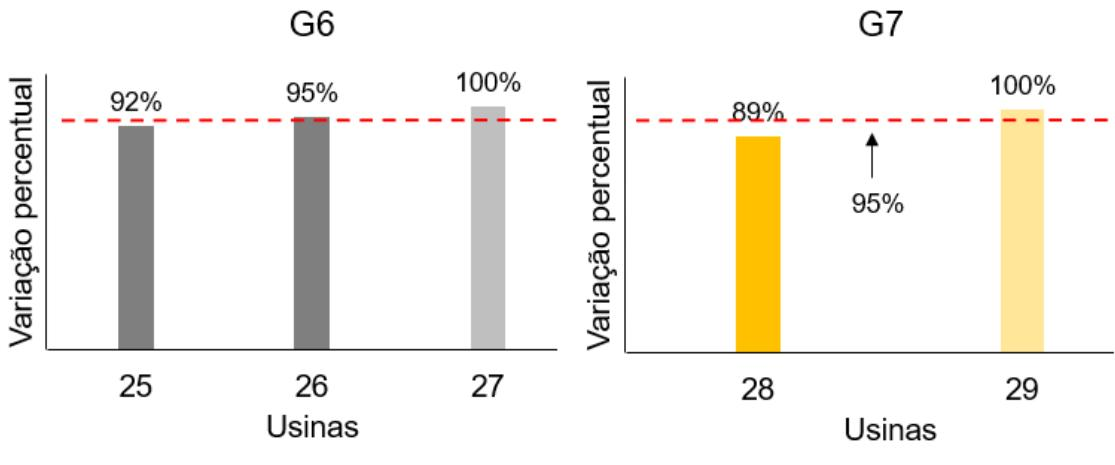
\includegraphics[scale=0.35]{figuras/fig1.jpg}
	\end{center}
    \label{grafico}
	\centering Fonte: \citeonline{FAZAL2023}
\end{figura}

Para referenciar o objeto inserido, utilize ``$\backslash$autoref\{\}''. Resultando em algo do tipo: ``Na \underline{\autoref{grafico}}, vemos que\ldots''. Caso clique no trecho sublinhado, o leitor é levado diretamente ao objeto referenciado (equação, figura, tabela, etc...).

É importante exportar imagens de boa qualidade ou em formato vetorial. Isso aumenta a qualidade da imagem no documento e permite, por exemplo, dar zoom na página sem perder o foco.

Para mais alguns comandos sobre imagens, pode acessar a página ``\textit{Como adicionar figuras em LaTeX – CL 6}'', de autoria do Felipe Cabral, clicando \href{https://vidaestudantil.com/podcasts/como-adicionar-figuras-em-latex-cl-6/}{\underline{\textit{\textbf{aqui}}}}.

\noindent \textbf{Tabelas}

As tabelas contém apenas linhas horizontais e devem estar centralizadas no documento, sendo identificada com seu número e com uma legenda na sua parte superior.

Para inserir tabela precisa de um pouco mais de dedicação. Mas vou deixar dois exemplos ``simples''.

\begin{tabela}[h!b!tp]
    \caption{Pessoas residentes em domicílios particulares, por sexo e situação do domicílio - Brasil - 1980}
    \begin{center}
        \begin{tabular}{lccc>{\centering\arraybackslash}p{1.8cm}c}
        \specialrule{2pt}{0pt}{1pt}
        \hline
        Situação do Total & Total       & Mulheres   & Homens \\
        \specialrule{1pt}{1pt}{1pt}
        Total             & 117.960.301 & 59.595.332 & 58.364.969\\
        Urbana            & 79.972.931  & 41.115.439 & 38.857.492 \\
        Rural             & 37.987.370  & 18.479.893 & 19.507.477 \\
        \specialrule{2pt}{0pt}{0pt}
        \hline
        \end{tabular}\\
    \end{center}
    \centering Fonte: IBGE (2013)
    \label{tab:Residentes}
\end{tabela}

O primeiro é uma tabela simples (\autoref{tab:Residentes}), com 4 linhas e 4 colunas. As bordas superior e inferior estão destacadas com uma espessura de linha um pouco superior em relação a linha que separa o título das demais linhas.

O segundo exemplo de tabela que vale a pena passar para vocês (e que eu passei muito tempo quebrando a cabeça para tentar fazer), é aquelas que dispões de células com quebra de texto. Vou deixar um exemplo abaixo (\autoref{tab:Comparativo dos dispositivos}) que utilizei em um dos meus trabalhos.

\begin{tabela}[h!b!tp]
    \caption{Comparação entre os dispositivos}
    \begin{center}
        \begin{tabular}{lccc>{\centering\arraybackslash}p{1.8cm}c}
        \specialrule{2pt}{0pt}{0pt}
        \hline
        Modelo & \makecell{Potência\\Ativa\\Total} & \makecell{Potência\\Reativa\\Total} & \makecell{Potência Ativa\\e Reativa\\(fundamentais)} & \makecell{Tensão e\\Corrente\\RMS} & \makecell{Variação de\\Corrente} \\
        \hline
        ADE7858A & Sim & Sim & Não & Sim & Sim \\
        ADE7868A & Sim & Sim & Não & Sim & Sim \\
        ADE7878A & Sim & Sim & Sim & Sim & Sim \\
        \specialrule{2pt}{0pt}{0pt}
        \hline
        \end{tabular}\\
    \end{center}
    \centering Fonte: Adaptado de \citeonline{ade78xxa}.
    \label{tab:Comparativo dos dispositivos}
\end{tabela}

Uma dica preciosa é que, caso ache difícil fazer as tabelas em LaTeX, pode fazer em outro software e realizar o upload para a plataforma (indico bastante o formato EPS para TODAS as imagens que forem utilizar no Overleaf). Feito isso, para identificar que se trata de uma tabela, basta seguir os comandos que constam no arquivo ``\textit{3-materiais e metodos.tex}''. %Os comandos se encontram logo abaixo desse parágrafo (mas não vão aparecer nesse PDF, então visualizem o arquivo .tex que mencionei antes). Já o resultado você pode observar na \autoref{tab:figtabela}.

\begin{tabela}[h!b!tp]
    \caption{Exemplo de tabela importada como imagem (igual a \autoref{tab:Comparativo dos dispositivos}, mas é uma imagem feita em outro software)}
    \begin{center}
        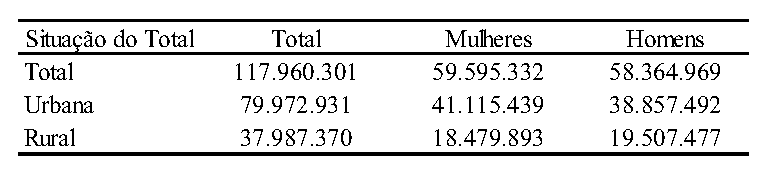
\includegraphics{figuras/figtabela.eps}
    \end{center}
    \centering Fonte: IBGE (2013)
    \label{tab:figtabela}
\end{tabela}

Certamente elementos como tamanho, formatação, letras, entre outros, da \autoref{tab:figtabela} está um pouco diferente da \autoref{tab:Residentes}. Mas a essência era mostrar que dava pra fazer a tabela em um software, mandar para um editor de imagens, exportar para o Overleaf e plotar como se fosse uma tabela (que foi exatamente o que eu fiz).

No meu caso, fiz a tabela no Excel, copiei para o CorelDRAW e exportei a imagem em formato EPS .

Mas se mesmo assim quiser fazer as tabelas aqui no Overleaf mesmo, para ensinar melhor sobre tabelas, vou indicar a página ``\textit{Como escrever tabelas em LaTeX – CL 7}'' que como sugere o título fala sobre sobre construção de tabelas em LaTeX. A página pode ser acessada clicando \href{https://vidaestudantil.com/podcasts/como-escrever-tabelas-em-latex-cl-7/}{\underline{\textit{\textbf{aqui}}}}. Também existem ferramentas online que convertem arquivos Excel parra LaTeX e/ou permitem que faça uma tabela nela própria, como por exemplo o site ``Converter Excel em LaTeX tabela'' (nome bem sugestivo) e que pode ser acessado clicando \href{https://tableconvert.com/pt/excel-to-latex}{\underline{\textit{\textbf{aqui}}}}. Para outros exemplos, basta realizar uma pesquisa rápida no Google que consegue achar vários resultados (alguns funcionais e simples, outros não).\vspace{0.2cm}

\noindent \textbf{Diagramas}

Diagrama é uma representação gráfica usada para demonstrar um esquema simplificado. Em elétrica, por exemplo, utilizamos para realizar a representação gráfica de circuitos elétricos e eletrônicos.

Abaixo tem um exemplo de diagrama.

\begin{diagrama}
    \caption{Caption}
    
\includegraphics[width=100mm]{figuras/diagramaBlocos.eps}\\
    \centering Fonte: \citeonline{batista2015}
    \label{fig:VSGDSC}
\end{diagrama}

Eu acho que todas as dicas para apresentar esse modelo em LaTeX já foram feitas. Quaisquer outras dúvidas podem ser sanadas pelo meu \href{mailto:christian.araujo96@outlook.com}{e-mail}, Google, Bing, ChatGPT, Google Bard, YouTube, etc...